\documentclass {article}

\usepackage[utf8]{inputenc}
\usepackage{lmodern}
\usepackage[T1]{fontenc}
\usepackage{graphicx}
\usepackage[official]{eurosym}
\usepackage{subcaption}
\usepackage[hidelinks]{hyperref}
\usepackage[italian]{babel}
\usepackage[backend=bibtex8, sorting=none]{biblatex}

\addbibresource {database.bib}

\graphicspath { {./media/} }
%TODO:EMPOOL + GRAFICO, PRIVATE KEY (QUANTE, RELAZIONE CON PUBLIC), N TOT ADDRESSES O KEYS, PROBABILITA(WIKI)BLOCCHI

\begin{document}

\begin{titlepage}

\centering
{\Huge Bitcoin, Blockchain, Crypto\par}
\vfill
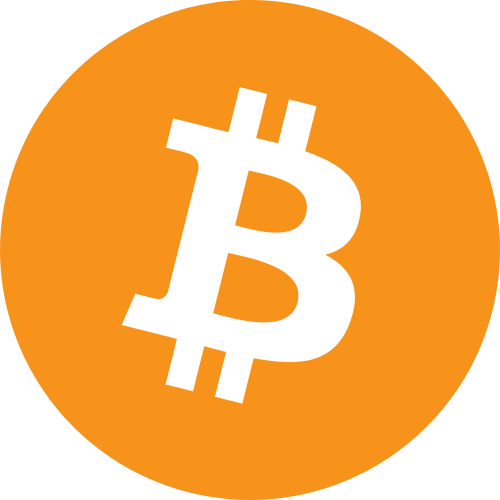
\includegraphics [width = 6cm] {logo.png}
\vfill
{\LARGE Carlomaria Occhipinti 5F\par}
\vspace{1cm}
{\Large Liceo Scientifico Arturo Tosi \par}
\vspace{1cm}

\end{titlepage}

\pagenumbering {gobble}

\newpage

\tableofcontents
\pagenumbering {arabic}

\newpage


\section {Le origini del Bitcoin}


2009. Il mondo è sconvolto dalla catastrofica crisi dell'anno precedente.
L'economia era in distruzione. Banche, borse e stati sull'orlo del crollo. Panico.
C'era il bisogno di una soluzione a tutto questo. Un sistema monetario che fosse immune a tutto ciò che colpì le valute crollate. Il Bitcoin\footnote{Nella tesina scriverò "Bitcoin" con la 'B' maiuscola per riferirmi alla valuta in generale, mentre con "bitcoin" con la 'b' minuscola mi riferisco ai bitcoin in sé, la moneta usata per fare acquisti, per esempio "5 bitcoin"}, la prima criptovaluta del mondo creata a cavallo tra il 2008 e il 2009 fu la risposta a tutti questi problemi economici legati alla crisi.

\paragraph {Satoshi}

Satoshi Nakamoto è conosciuto come l'ideatore e l'iniziale sviluppatore del Bitcoin.
L'identità di Satoshi è una questione discussa da sempre, e certi individui sono sospettati di essere il creatore del Bitcoin.
In realtà nessuno sa veramente chi sia, dove abiti, se è un singolo o un gruppo di persone. Sappiamo solo che nei primi anni del Bitcoin era attivo sul forum bitcointalk.org fino al 13 dicembre 2010. e che il 31 ottobre 2008 Satoshi scrisse il \textit{whitepaper}\footnote{"Libro bianco", un documento redatto da un professionista esperto di una materia che offre informazioni di qualità e di interesse ad un pubblico selezionato di utenti.} del Bitcoin contenente la sua ideologia di moneta virtuale.
Il documento è altamente tecnico e richiede un'elevata conoscenza di informatica e matematica, perciò ritengo superfluo citarne delle parti. \cite{whitepaper}

\paragraph {Confronto con i soldi "tradizionali"}

Il Bitcoin si differenzia radicalmente dalla moneta legale\footnote{Chiamata anche "fiat" (da non confondersi con la casa di automobili)}.
Esso è:

\begin{itemize}
\item Decentralizzato: è una valuta internazionale, non legata particolarmente ad alcun paese (come lo Yen col Giappone, il Franco con la Svizzera). Le transazioni sono \textit{peer-to-peer}, da pari a pari, senza la necessità di passare da un ente centrale come una banca.
\item Deflazionario: la quantità totale limitata di bitcoin impedisce la perdita di valore della valuta, cosa che avviene frequentemente con le monete legali artificialmente inflazionate.
\item Anonimo: non sono richieste informazioni personali per inviare e ricevere Bitcoin, per questo si ha una maggior tutela della privacy.
\item Veloce: la natura \textit{peer-to-peer} della valuta rimuove tutti gli eventuali ritardi e complicazioni che si possono avere con un gestore di carta di credito.
\end{itemize}


\newpage


\section {Blockchain: cos'è e come funziona}


La tecnologia rivoluzionaria utilizzata dal Bitcoin e da tutte le altre criptovalute è chiamata Blockchain.
Come suggerisce il nome, "blockchain" indica una catena di blocchi.
L'aspetto decentralizzato del Bitcoin gira intorno al fatto che chiunque può scaricare la blockchain e far sì che si aggiorni in tempo reale: ciò significa che finché esiste in tutto il mondo \emph{almeno} un computer con la blockchain salvata, che prende il nome di \textit{full node}, l'intera rete del Bitcoin e il registro delle transazioni rimangono autentiche e inviolate nella maggior parte dei casi (vedi X.X).

\vspace {0.5cm}
\begin{figure}[htb!]
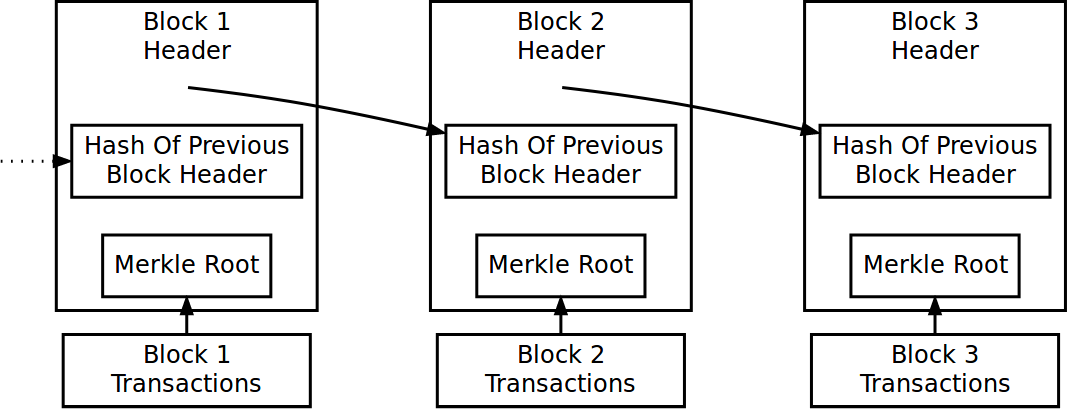
\includegraphics [width = 10cm] {blockchain2.png}
\centering
\caption {Schema della blockchain\\\textit{fonte: bitcoin.org}}
\end{figure}


\subsection {Cosa sono i blocchi e che compito svolgono}

Ciascun blocco contiene informazioni sulle transazioni di bitcoin che sono state effettuate di recente.
Il blocco può essere visto come un contenitore, un hard disk grande 1MB che contiene un determinato numero di transazioni.
Le transazioni hanno un determinato peso espresso per comodità in kilobyte fare paragrafo mempool+foto, dove lo metto? (domanda:come fanno le transazioni ad essere messe nei blocchi?)
Tutte le transazioni di Bitcoin sono permanentemente, irreversibilmente (nella maggior parte dei casi, V X.X) memorizzate nella Blockchain.
Su un qualunque sito avente la funzione di "block explorer" posso cercare informazioni su ciascun indirizzo Bitcoin (per ora pensiamolo come se fosse un codice IBAN): posso vedere quanti Bitcoin quell'indirizzo possiede, da quali indirizzi ha ricevuto quanti bitcoin, e a chi ne ha mandati.
Sotto un punto di vista pratico, la blockchain del Bitcoin è un file di dimensioni oggi pari a circa 170 Gigabyte.
La dimensione è così elevata perché in quel file sono contenute le informazioni di oltre 520.000 blocchi scoperti a partire dal primo, chiamato \textit{genesis block}, trovato il 3 gennaio 2009.
"Scoperti"? "Trovati"? In che senso? Da dove vengono questi blocchi? Mi tocca introdurre il concetto di \textit{mining}.


\subsection {Mining}


Sebbene non sia tecnicamente corretto, il modo più semplice per spiegare il concetto di \textit{mining} è quello di paragonare i bitcoin a una montagna nella cui roccia sono contenuti minerali preziosi.
I bitcoin sono, per esempio, l'oro nella roccia.
Per trovare l'oro bisogna scavare nella roccia della montagna utilizzando speciali apparecchiature quali ruspe, trapani, trivelle.
I blocchi, per poter essere "scoperti" vengono "minati" dai cosiddetti miner ASIC (\textit{application specific integrated circuit}), dei computer specializzati a risolvere un certo tipo di algoritmo che nel \textit{whitepaper} Satoshi definisce come \textit{proof of work}\footnote{Abbreviato "PoW", tradotto "prova di lavoro" o "prova di funzionamento"}: la PoW è l'algoritmo usato dal Bitcoin per confermare le transazioni e avanzare al blocco successivo della blockchain.
Esso si basa sulla risoluzione di un problema matematico difficile (descritto nei paragrafi successivi) compiuta dai miners per poter ottenere una soluzione facilmente verificabile dai \textit{full nodes} in tutto il mondo.
Lo scopo della \textit{proof of work} e il motivo per cui è presente un difficile problema matematico da risolvere è quello di impedire la generazione illimitata di blocchi e di conseguenza di abusare della blockchain .

\paragraph {Le hash}

L'obiettivo del mining è quello di indovinare una "parola chiave", chiamata \textit{hash}, una serie di numeri e lettere che serve per trovare un blocco.
Il Bitcoin usa l'algoritmo SHA-256, quindi le hash indovinate dai miner sono lunghe 64 caratteri.
Questo perché come suggerisce il nome, 256 indica il numero di \textit{bits} che costituiscono la stringa.
Il \textit{bit} è la più piccola unità di misura per quanto riguarda la dimensione di file nel campo dell'informatica, e 8 bit corrispondono a 1 byte.
Nel sistema numerico esadecimale un carattere "pesa" 8 bit, quindi $256 : 8 = 64$.
Una hash facente parte dell'algoritmo SHA-256 non può essere una qualunque combinazione di 64 numeri e lettere, ma deve rispettare determinati parametri per essere considerata tale, di cui non scriverò per evitare di complicare ulteriormente la situazione.
In succinto, per trovare il numero di hash totali che si possono ottenere bisogna effettuare il  calcolo $2^{256}$, che corrisponde a circa $1,158 \times 10^{77}$ possibili hash da indovinare.
Le hash che portano alla scoperta di uno specifico blocco, però, possono essere più di una.

\subsubsection {Target e difficoltà di mining}

Per trovare un blocco è necessario che i miners trovino un'\textit{hash} che sia inferiore al cosiddetto \textit{target}. Il target è un'hash che fa da "confine" sotto al quale tutte le hash sono accettabili.
Tutte le hash trovate dai miners che hanno valore minore del target sono valide, e portano alla scoperta di un nuovo blocco.
Con "difficoltà" si intende, ovviamente, quanto è difficile trovare un blocco, e il suo valore è collegato a quello del target.
Più si abbassa il target, più si alza la difficoltà, perché abbassandosi il target le hash valide diventano meno, quindi la probabilità che i miners ne trovino una valida si riduce.
Ma perché dovrebbe abbassarsi il target?

Man mano che sempre più miners cominciano a lavorare, elevando l'\textit{hashing power} complessivo del network del Bitcoin, se non ci fossero cambi di target i blocchi verrebbero trovati con frequenza sempre più elevata.

\vspace {0.5cm}
\begin{figure}[htb!]
\makebox [\textwidth] [c] {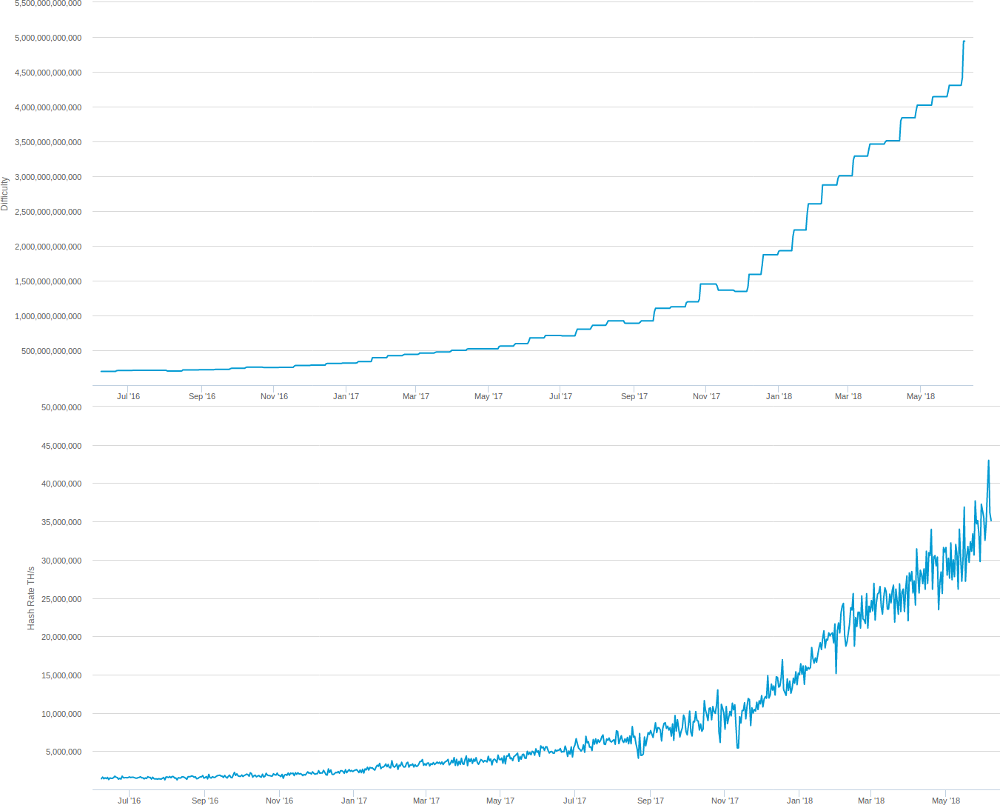
\includegraphics [width=15cm] {hashdiff.png}}
\caption {Confronto tra difficoltà (sopra) e hashrate globale (sotto)\\\textit{fonte: blockchain.info}}
\end{figure}
\vspace {0.2cm}
\noindent
%
L'innalzamento o talvolta anche l'abbassamento della difficoltà avviene ogni 2016 blocchi (circa 2 settimane), quando il network controlla la frequenza con cui questi ultimi blocchi sono stati trovati.
Modificando la difficoltà in modo proporzionale all'\textit{hashing power} si fa in modo che in media i blocchi continuino ad essere trovati ogni \textasciitilde 10 minuti. Perché 10 minuti?

\paragraph {Tempo per blocco}

Satoshi ha deciso che ogni blocco deve impiegare un tempo di circa 10 minuti per essere scoperto.
Il motivo della scelta è quello di aver trovato un compromesso: sacrificare conferme e quindi transazioni più veloci per avere un processo di mining più efficiente.
Nell'intervallo di 10 minuti tutti i \textit{full nodes} hanno tempo sufficiente per accettare e validare l'ultimo blocco trovato e far sì che si propaghi in tutta la rete, impedendo eventuali conflitti su qual è la blockchain autentica. %more bandwith??
Quando non avviene ciò, può capitare che fra due blocchi che vengono trovati in istanti vicini solo uno dei due venga accettato dalla maggioranza dei \textit{full nodes}.
Il blocco che viene abbandonato è definito \textit{stale block}\footnote{Blocco in stallo}, ovvero un blocco inizialmente considerato valido, ma poi abbandonato perché l'altro blocco trovato è stato accettato più velocemente, dando origine alla blockchain più lunga tra le due, quindi quella più reputabile.
Per questo con i blocchi di 10 minuti si ha un mining più efficiente, perché si riduce la quantità di energia elettrica sprecata per far funzionare dei miners che trovano un blocco orfano.
Quando viene trovato un blocco, tutti i miners devono interrompere la ricerca del blocco ormai trovato e cominciare a lavorare su quello successivo.
Se questi non si fermano, troveranno eventualmente un blocco che è gia stato trovato, e che quindi non può essere "attaccato" alla blockchain.
Un blocco orfano, \textit{orphan block}, invece, è un blocco minato da un miner che non può essere accettato nella blockchain perché il \textit{node} del miner non si è ancora aggiornato alla blockchain più recente che include il blocco precedente a quello appena trovato.
Non avendo un "genitore" (\textit{parent}), il blocco trovato dal miner non viene propagato agli altri \textit{full nodes} perché non è "collegato" ad altri blocchi.
A partire dalla versione 0.10 del software del Bitcoin, però, non possono più esistere blocchi orfani a seguito di una modifica radicale del sistema con cui i \textit{nodes} scaricano i nuovi blocchi \cite{staleorphans}.

\vspace {0.5cm}
\begin{figure}[htb!]
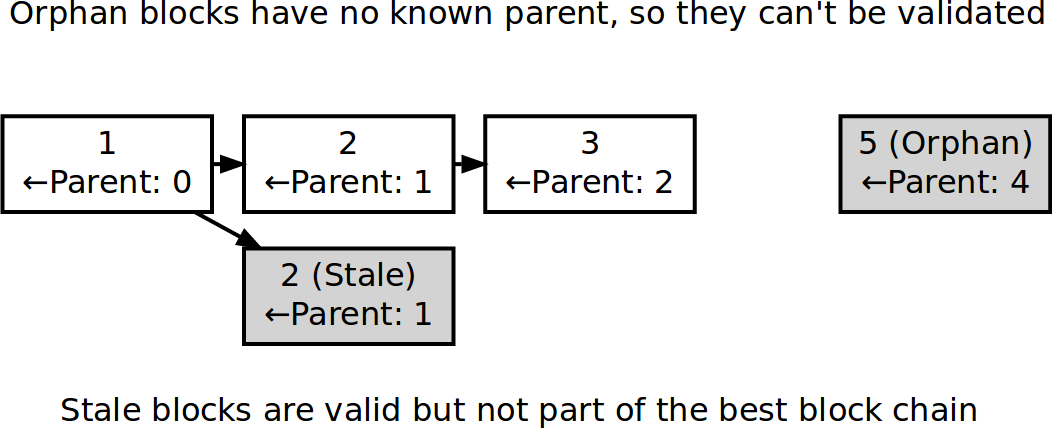
\includegraphics [width = 10cm] {stale-orphan.png}
\centering
\caption {Rappresentazione di blocchi in stallo e orfani}
\end{figure}
\vspace {0.2cm}
\noindent
%
Il tempo di 10 minuti di certo riduce la probabilità che vengano creati blocchi in stallo; tuttavia è sempre possibile che nascano.

\subsubsection {Costi del mining}

I miner di Bitcoin che si usano oggi lavorano a velocità comprese tra i 10 e i 14 TH/s (tera-hash al secondo) in base al loro consumo energetico, ovvero a oltre dieci trilioni di hash trovate in un secondo.
Questi apparecchi sono molto costosi (quelli di ultima generazione superano i \euro{700} per unità) e utilizzano un'elevata quantità di energia elettrica per funzionare.
Perchè, allora, c'è gente che spende tutti questi soldi per fare il lavoro di mining?
Ebbene, quando si trova un blocco, oggi il miner riceve una quantità pari a 12.5 BTC, pari a circa \euro{90.000} secondo il prezzo attuale.
Quasi mai, però, la \textit{block reward} finisce a una singola persona: indovinare l'hash che trova il blocco è estremamente difficile!
Per questo esistono le \textit{pool} di mining.

\paragraph {L'uso di elettricità del mining}

I miner ASIC usano una notevole quantità di energia. Prendendo in considerazione quelli di ultima generazione, il più potente, il Bitmain Antminer S9 (14 TH/s) consuma circa 1300 W, il più debole (4 TH/s) 1000 W.
In media, un S9 che lavora in una \textit{pool} di mining fa guadagnare circa 0.00082 BTC al giorno, ovvero circa \euro{5.5}.
Considerando che le \textit{farm} sono locate in paesi in cui l'elettricità costa poco, intorno ai \euro{0.04}/KWh, un S9 costa circa \euro{1} al giorno in elettricità.
Un miner, quindi, fa guadagnare almeno \euro{4} al giorno considerando il costo dell'elettricità.
Ho già scritto che i miner hanno un prezzo notevole, infatti un Antminer S9 costa attualmente \textasciitilde \euro{717}.
Prima di cominciare a guadagnare un profitto nel mining, bisogna calcolare il tempo impiegato per coprire il costo dell'attrezzatura di mining.
Questo tempo si chiama ROI \footnote{\textit{Return on investment}}, e nel caso della situazione presa come esempio, ovvero quella di guadagnare \euro{4} al giorno con un S9, il ROI è pari a 179 giorni, infatti

$$\textup{\euro{717}} : \frac{\textup{\euro{4}}}{1 giorno} = 179.25 giorni$$
%
Questo è quanto vale per \emph{un} singolo ASIC che produce solo 0.00082 BTC al giorno, una quantità minuscola rispetto ai \textasciitilde 17.000.000 che sono stati minati fino ad oggi.
L'\textit{hashing power} dell'intero network del Bitcoin, la somma del lavoro dei miners in tutto il mondo espressa in H/s, è di oltre 30.000 TH/s, e consuma un a quantità di elettricità pari a 60 TWh, ovvero 60.000 miliardi di Joule consumati all'ora.
Questo consumo di elettricità corrisponde a (piu di 0.13, perche dati dic 2017, cercare nuovi) dell'utilizzo di elettricità in tutto il mondo.
... ... ... (citazione a powercompare.co.uk)


\subsubsection {Profitti del mining}


Perchè, allora, c'è gente che spende tutti questi soldi per fare il lavoro di mining? (lo metto prima o dopo inizio sezione?)
Ebbene, quando si trova un blocco, oggi il miner riceve una quantità pari a 12.5 BTC, pari a circa \euro{90.000} secondo il prezzo attuale.
Quasi mai, però, la \textit{block reward} finisce a una singola persona: indovinare l'hash che trova il blocco è estremamente difficile!
Per questo esistono le \textit{pool} di mining.

\paragraph {Mining pools}

Le \textit{pool} sono dei siti in cui più miners\footnote{Con "miner" ci si può riferire sia ai computer che compiono il lavoro, sia alle persone che li operano e che guadagnano bitcoin} uniscono gli sforzi per trovare un blocco.
Nella configurazione del software che fa compiere il mining agli ASIC bisogna inserire l'indirizzo web della \textit{pool} per la quale si vuole lavorare, e il miner comincierà ad inviare le hash che calcola alla pool.
Una volta trovato il blocco, la ricompensa di bitcoin si spartisce fra tutti i miner, in base a quanto ciascuno si è impegnato per trovarla.
È possibile controllare il lavoro dei miners tramite un'interfaccia remota. Su tutti i siti delle \textit{pool} è possibile inserire in un campo di ricerca l'indirizzo Bitcoin verso cui i bitcoin ricavati saranno inviati.

\vspace {0.5cm}
\begin{figure}[htb!]
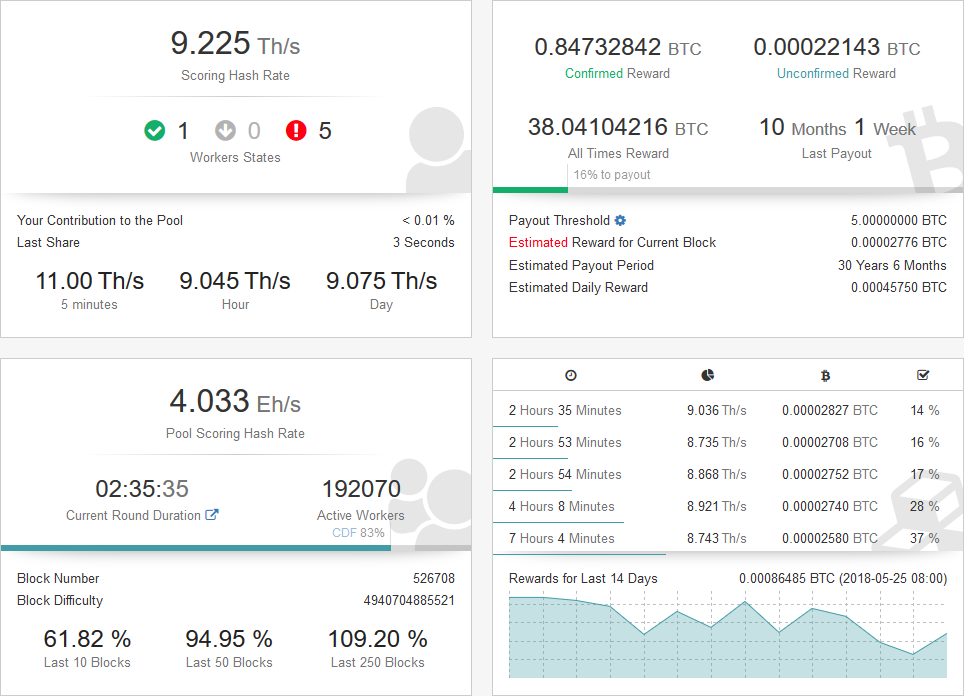
\includegraphics [width = 10cm] {dashboard.png}
\centering
\caption {Interfaccia di una \textit{mining pool}: si possono scorgere hashrate (in alto a sinistra), bitcoin guadagnati e le stime sui guadagni giornalieri e il tempo rimanente per ricevere il pagamento (in alto a destra)\\\textit{fonte: slushpool.com/dashboard}}
\end{figure}
\vspace {0.2cm}

\paragraph {Tassa di transazione}

La scoperta dei blocchi non è l'unico metodo con cui coloro che praticano mining guadagnano Bitcoin.
Ogni transazione di Bitcoin prevede il pagamento di una piccola quota, solitamente compresa tra \euro{0.01} e \euro{1}.
Questa quota, chiamata \textit{miner fee} serve per incoraggiare i miner a selezionare la nostra transazione da includere nel blocco in fase di ricerca.
Questa tassa/commissione è espressa in sat/byte, satoshi\footnote{Un satoshi è l'unità di misura più piccola del bitcoin, e corrisponde a $1 \times 10^{-8}$ BTC} per byte.
Una tassa più elevata riduce il tempo di conferma della transazione, perché preferita dai miner. Al contrario, una transazione effettuata con una tassa inferiore alla media impiega più tempo ad essere inclusa in un blocco e quindi ad essere processata, perché i miner guadagnano più BTC dalle transazioni più costose.
Come ho spiegato ciascuna transazione pesa tot kilobyte, quindi, conoscendo il peso in kb della transazione e avendo stabilito il valore della tassa in sat/byte\footnote{Spiegherò come si viene a conoscenza di queste due nel punto X.Y} per scoprire quanto paghiamo effettivamente possiamo ricavare la quantità di BTC dalla proporzione.

$$ nSatoshi : 1 byte = tassa : pesoTransazione $$
%
o semplicemente utilizzando la formula $x tassa = \frac{nSatoshi \times pesoTransazione}{1 byte}$.

\paragraph {Il futuro del mining}

In precendenza ho detto che la scoperta di un blocco porta al guadagno dei miners di 12.5 BTC.
Questa ricompensa, però, non è un valore costante: ogni 210.000 blocchi trovati la quantità di bitcoin che i miners ricevono si dimezza, infatti la ricompensa iniziale era di ben 50 BTC. Questo processo di dimezzamento è chiamato \textit{halving}.
Oggi abbiamo superato il blocco numero 526000, infatti essendo 526.000 : 210.000 = \textasciitilde 2.5, fin ora ci sono stati due \textit{halving}.
50 : 2 = 25, 25 : 2 = 12.5, la ricompensa attuale.
I bitcoin, però, esistono in quantità limitata, infatti il limite massimo è di 21.000.000 BTC.
Fino ad oggi sono stati minati circa 17.000.000 BTC, ovvero l'81\% della quantità totale.
Eventualmente tutti i bitcoin verranno minati, e i profitti dei miners dipenderanno esclusivamente dalle tasse di transazione.


\newpage


\section {Aspetto tecnico del Bitcoin}


\subsection {Mempool: il primo passo delle transazioni}


La mempool si è dove stanno le tx non confermate ma sempre nei full nodes...


\subsection {Come e dove si conserva}


\subsubsection {Indirizzi}


Poiché i bitcoin non sono oggetti materiali, si dice che nella blockchain sono associati X BTC a ciascun indirizzo.
sono presenti tanti tanti (numero tot indirizi?)
Gli indirizzi sono delle stringhe di circa 30/40 caratteri che possono essere visti come codici IBAN se si vuole rimanere in un contesto finanziario, o anche come indirizzi email.
Esistono diversi tipi di indirizzo.

\paragraph {P2PKH}

Gli indirizzi P2PKH "\textit{Pay To PubKey Hash}", comunemente chiamati indirizzi "legacy", sono il primo formato di indirizzo, utilizzato esclusivamente fino all'agosto del 2017.
Questi indirizzi si riconoscono dal fatto che iniziano col carattere '1', per esempio \texttt{12dmWhp2dyog8GQRX3GMFqmFmV3duWUMmN}.

\paragraph {P2SH SegWit}

P2SH significa "Pay 2 Script Hash".
Gli indirizzi P2SH sono stati ideati il 18 ottobre del 2011 con il BIP-13 e mandati live l'1 Aprile del 2012.
Il lancio di questi indirizzi non avvenne affatto in modo liscio e "indolore": il problema principale è che tutti i miners che non hanno aggiornato il proprio \textit{full node} stavano includendo nei blocchi transazioni ritenute invalide dai loro software.
La differenza sostanziale con gli indirizzi "normali" è che ..multisig...sigh...è difficile

\paragraph {bech32 SegWit}

Gli indirizzi Bitcoin bech32 implementano SegWit al 100\%, e di conseguenza sono quelli con le tasse di transazione/i più inferiori.
Questo tipo di indirizzo è stato creato nel XXXX, ed essendo sotto un punto di vista tecnico molto diverso dagli indirizzi tradizionali (che cominciano con 1 e 3), non sono supportati da una moltitudine di siti di compravendita e da portafogli, (di cui parlerò in seguito).
Gli indirizzi bech32, infatti, hanno il prefisso "bc1", e tutt'oggi cose


\subsubsection {Keys}


Ogni indirizzo Bitcoin è composto due chiavi: una \textit{public key} e una \textit{private key}. dovementtto come si generano e che ne esistono un casino?

\paragraph {Public key}

Da non confondere con l'indirizzo in sé, la chiave pubblica(key lo dico in ing o ita?), la chiave pubblica è una forma diversa dell'indirizzo.
L'indirizzo è la chiave pubblica \textit{hashata}, per questo è di dimensioni più corte. (impreciso, sistemo).
%Every public key is 256 bits long — sorry, this is mathematical stuff — and the final hash (your wallet address) is 160 bits long.
%The public key is used to ensure you are the owner of an address that can receive funds.
%The public key is also mathematically derived from your private key, but using reverse mathematics to derive the private key would take the world’s most powerful %supercomputer many trillion years to crack.
%dal sito dei dammis. quando dico n tot indiriziz? dopo devo anche scrivere di come funziona lo storage offline (come indirizzo email che puo ricevere ma non mandare v preferiti windows

\paragraph {Private key}

La \textit{private key} è un codice che consente a chiunque di avere accesso ai Bitcoin conservati nell'indirizzo.
Come le \textit{hash} viste in precendenza, le private key sono numeri di 256 \textit{bit}, che nel sistema numerico esadecimale sono codici di 64 caratteri tra numeri e lettere.
A differenza delle \textit{hash} SHA-256, però, le private key devono essere comprese tra ... ... 
È paragonabile ad una password che dà accesso ad account di qualunque tipo, l'unica differenza è che non è modificabile.

\paragraph {Seeds}

Un \textit{seed} è un codice che svolge una funzione simile a quella della \textit{private key}: se inserito in un software di wallet, ripristina tutti i bitcoin associati ad esso.
La differenza con le \textit{private keys} è che un seed "genera" una o più private keys, dalle quali si possono ricavare le public keys e quindi gli indirizzi stessi.
Di conseguenza, ad un seed possono corrispondere un numero indefinito di indirizzi, ovvero di coppie di public e private keys.
Realisticamente, quasi tutti i seed usati nei portafogli software comprendono da 1 a 20 indirizzi.
Esistono diversi tipi di seed, ma il formato più famoso è quello della cosiddetta \textit{mnemonic phrase}, una frase di 12 - 20 parole, introdotta nel 2 febbraio 2012 con il BIP-32.
Con il BIP-39 \footnote{\textit{Bitcoin Improvement Proposal}} è stato introdotto...?
Il vantaggio dei seeds rispetto alle singole private keys è il fatto che sono facili da ricordare. Un seed ha un aspetto simile al seguente:

\begin{quote}

witch color pride feed shame open despair creek road again ice least

\end{quote}
%
Il secondo vantaggio è che la presenza di molteplici indirizzi Bitcoin aiuta a tutelare la propria privacy.
Come abbiamo visto nella blockchain chiunque può accedere alle informazioni di chiunque (suona male), così per rendere i fondi meno tracciabili si possono usare diversi indirizzi per diverse operazioni.


\subsubsection {Portafogli}


Un portafoglio è il metodo usato per conservare e interagire con i Bitcoin che si possiede.
I portafogli contengono le chiavi pubbliche e private e di conseguenza l'indirizzo stesso.

\paragraph {Cold storage}

Con il \textit{cold storage}\footnote{Archiviazione a freddo}, \textit{public} e \textit{private} keys sono conservate offline, ovvero in un ambiente non collegato a internet.
Sebbene sia necessaria una connessione ad internet per effettuare transazioni, riceverle non la richiede (suona male).
(metto sopra?) quando creiamo un indirizzo a partire da una \textit{private key} ricavata casualmente, questo è in realtà già esistente nella blockchain.
Tutti gli indirizzi, \textit{public} e \textit{private} keys sono già esistenti nella blockchain a prescindere, e creando un indirizzo non stiamo facendo altro che appropriarcene di uno a caso.
È naturale porsi la domanda: "Ma se qualcuno "ottenesse" la mia private key mi ruberebbe tutti i soldi! Non è rischioso?".
Ebbene, come ho scritto prima, esistono X keys, un numero simile a 1/3 degli atomi in tutto l'universo. La probabilità è praticamente nulla. (riguardare, forse sbagliato e confondendo).
I principali tipi di \textit{cold storage} sono:

\begin{itemize}
\item Digitale: le keys sono salvate sottoforma di file su un computer, un CD, una chiavetta USB...
\item Carta: si possono scrivere le keys su un pezzo di carta o stampare un \textit{paper wallet}, metodo poco sicuro per la fragilità del materiale.
\item Metallo: le keys possono essere incise su una lamina di metallo, preferibilmente oro, argento, bronzo, nickel, ottone o cobalto per la resistenza alle alte temperature.
\item \textit{Hardware wallet}: I portafogli hardware sono dei piccoli dispositivi simili a chiavette USB, in cui la \textit{private key} è contenuta.
\end{itemize}

\begin{figure}[htb!]

\makebox [\textwidth] [c] { 
    \begin{subfigure}{8cm}
    %\hspace{2cm}
    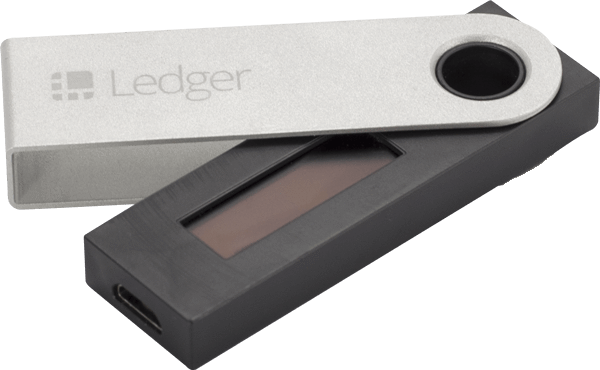
\includegraphics [height=4cm] {ledger.png}
    \caption{Un Ledger Nano S, portafoglio hardware}
    \end{subfigure}
    \begin{subfigure}{8cm}
    \makebox [\textwidth] [c] {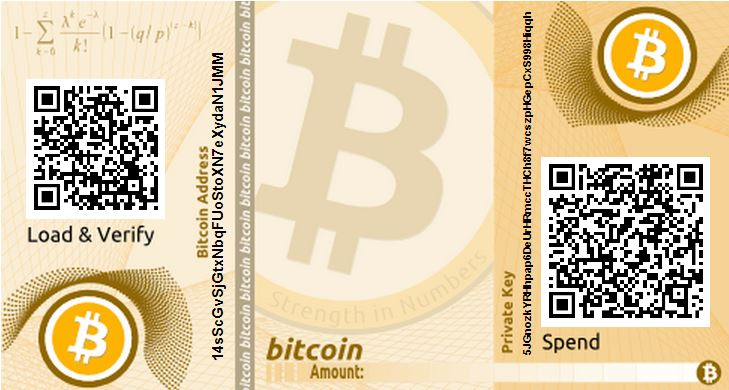
\includegraphics [height=4cm] {paper.jpg}}
    \caption{Un \textit{paper wallet}}
    \end{subfigure}
}
 
\caption{Due forme di \textit{cold storage}}

\end{figure}
\vspace {0.2cm}
\noindent
%
Esistono anche dei veri e propri "Bitcoin" fisici, ovvero delle monete materiali con incise le keys.
Hot wallets are like checking accounts while cold wallets are similar to savings accounts.x me poi tolgo

\paragraph {Hot wallets}

Gli \textit{hot wallets} sono invece dei portafogli che utilizzano un collegamento a internet per permettere di effettuare pagamenti \emph{dall'}indirizzo in uso.
Gli \textit{hot wallets} esistono come software, tra cui app per smartphone, programmi per computer o servizi online.


\subsection {I problemi del Bitcoin}


\subsubsection {Gli attacchi al network}


La rete del Bitcoin può essere abusata da malintenzionati per compiere \textit{double spending}, ovvero l'atto di spendere una stessa quantità di Bitcoin due volte, effettivamente annullando il primo pagamento.
Il \textit{double spending} è solitamente usato per truffare: dopo aver inviato \textit{x} BTC al ricevente, il truffatore fa subito un attacco di \textit{double spending} inviando a sé stesso la stessa quantità di bitcoin. Il ricevente si troverà con 0 BTC, che sono rimasti al truffatore.
Esistono quattro principali modi per fare \textit{double spending}: \cite{attacks}

\begin{itemize}
\item \textit{Race attack}:
\item \textit{Finney attack}:
\item \textit{Vector76 attack}:
\item \textit{Majority attack}: più comumemente conosciuto come "\textit{51\%}" o "\textit{>50\% attack}", è il tipo di attacco più temuto perché può essere applicato a qualunque transazione, indipendentemente dal numero di conferme ricevute\footnote{Ricordo che una conferma corrisponde a un blocco trovato dopo aver effettuato il pagamento. Più conferme rendono una transazione più sicura perché questa viene "superata" da un maggior numero di blocchi}.
Un attacco 51\% si può effettuare solo se un singolo possiede più della metà dell'\textit{hashrate} di tutta la rete del Bitcoin.
Dopo aver pagato il mercante, questo attende \textit{x} conferme e poi invia la sua merce.
Il truffatore sdoppia la blockchain e su questa ripete il pagamento a un indirizzo in suo controllo; in seguito impiega il 51\% dell'hashrate per minare blocchi sul suo clone privato della blockchain, e dopo aver trovato un numero di blocchi maggiore al numero di conferme attese manda "live" la sua blockchain ai \textit{full nodes} in tutto il mondo per sostituire quella più corta, nella quale il mercante aveva ricevuto bitcoin.
\end{itemize}


\subsubsection {La parziale centralizzazione}


L'intenzione di Satoshi, con la creazione della blockchain e di un sistema di mining universale, fu quella di creare una valuta decentralizzata, e in parte ci riuscì.
Purtroppo, il lavoro dei miners è concentrato in una piccolo gruppo di pools che possiedono quasi tutta l'\textit{hashrate} globale \cite{centralization}.

\vspace {0.5cm}
\begin{figure}[htb!]
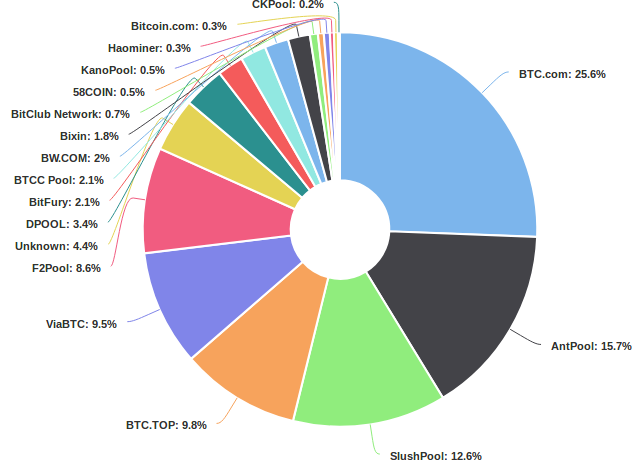
\includegraphics [width = 10cm] {pools.png}
\centering
\caption {pie-chart della percentuale di hashrate controllata dalle più grandi pool\\\textit{fonte: blockchain.info}}
\end{figure}
\vspace {0.2cm}
\noindent
%
Non ci sono \textit{pools} con una percentuale di \textit{hashrate} maggiore al 50\%, ma è sufficiente dirottarne 3 per compiere un attacco 51\%, essendo la maggior parte situate in Cina.


\subsubsection {Il limite dei blocchi da 1 Megabyte}



\paragraph {Segregated Witness}

Segregated Witness (comunemente abbreviato in SegWit) è una roba che riduce le tasse

\paragraph {Lightning Network}

Il Lightning Network è un network lightning.
infrastruttura esterna alla blockchain che rende cose veloci

\newpage


\section {Utilizzare Bitcoin}


Ho notato che nonostante se ne parli sempre di più in televisione e su internet, il Bitcoin è sempre visto come un concetto astratto, un'entità misteriosa di cui non si sa esattamente come si usa, dove si prende, e in cosa si spende.
In questa sezione spiegherò come entrare in contatto con l'ecosistema delle criptovalute, partendo dalla creazione di un portafoglio (\textit{hot} e non \textit{cold} per avere la possibilità di effettuare pagamenti).


\subsection {Creazione del portafoglio}


Come descritto in X.X, il portafoglio è quel software che ci dà l'accesso ai bitcoin salvati nella blockchain.
Per comodità è consigliabile usare un app per smartphone: sull'App Store dei dispositivi Apple e sul Play Store di quelli Android sono disponibili numerosi portafogli di Bitcoin, ma il funzionamento è lo stesso per tutti.
Una volta scaricato il portafoglio incomincia la creazione di un nuovo indirizzo che verrà usato per inviare e ricevere bitcoin.
L'app ci mostrerà il \textit{seed} al quale sono associati i nostri indirizzi (ma talvolta solo uno).
Il seed dovrà essere copiato e conservato in un luogo sicuro (su carta e/o chiavetta USB), perché nello sfortunato caso in cui perdiamo il nostro smartphone sarà possibile importarlo in un altro dispositivo.
Una volta confermato il seed saremo in grado di inviare e ricevere Bitcoin al nostro indirizzo.


\subsection {Come ottenere Bitcoin}


\paragraph {Exchange}


Il metodo più veloce e utilizzato è quello di acquistarlo su un sito di \textit{exchange}\footnote{"Scambio", siti di compravendita di valute}. Esistono moltissimi siti che permettono di acquistare Bitcoin con bonifico bancario o semplicemente con una carta di credito.
Coinbase è di gran lunga l'exchange più famosa del mondo, ma ne esistono una moltitudine.
Basta aprire un account, collegare il proprio conto o la carta di credito, verificare la propria identità con passaporto o carta d'identità e compare bitcoin è questione di secondi.
Una volta acquistato, è consigliabile spostare i propri bitcoin su un portafoglio indipendente da quello dell'exchange.
Quasi tutte le exchange più reputabili sono dotate di sistemi di sicurezza ad elevatissimo livello che riducono la possibilità di una violazione della sicurezza al minimo, ma ci sono stati tragici episodi di exchange colpite da attacchi hacker, derubate di quantità di bitcoin che oggi valgono milioni di Euro.
Ritengo che non valga la pena di rischiare di perdere tutti i propri bitcoin per la pigrizia di non volerli mettere al sicuro.

\paragraph {ATMs}

Esistono dei veri e propri "Bancomat" in cui anzichè prelevare soldi dal proprio conto bancario è possibile acquistare e vendere criptovalute.
Sono comodi, veloci ed anonimi, ma c'è sempre il rischio di venire derubati tramite forza fisica; si paga un bonus per la comodità e al giorno d'oggi sono ancora molto poco diffuse.
Si può trovare una mappa online con la posizione di questi ATM in tutto il mondo su coinatmradar.com.

\paragraph {Mining}

Come spiegato in precedenza, il processo di mining porta i miners a guadagnare Bitcoin, che possono essere venduti sulle exchange per soldi veri e propri.
Ovvio che per una persona inesperta il mining è fuori portata, ma è certamente un modo valido per ottenere Bitcoin.

\paragraph {Forma di pagamento}

Al posto di soldi in contanti o carta di credito è possibile accettare Bitcoin come forma di pagamento per merce o servizi offerti in vita reale e online.
Esistono infatti diversi sistemi automatizzati che consentono ai mercanti di accettare criptovalute velocemente e in sicurezza.
Coinbase Commerce, per esempio, si integra con i siti web mostrando un'interfaccia di pagamento che permette di scegliere la criptovaluta con cui pagare e l'indirizzo verso cui pagare. Il pagamento è concluso solo quando Coinbase riceve il pagamento della quota, che reindirizza al portafoglio del mercante


\subsection {Trasferire Bitcoin}


Un tipico trasferimento da persona a persona avviene con gli smartphone.
Il ricevente va nella sezione "ricevi" della propria app, che gli mostrerà un codice QR che decifrato corrisponde all'indirizzo di pagamento.
Il pagatore va nella sezione (che brutto) "paga", e tramite la fotocamera del proprio telefono scansiona il codice QR del ricevente.
Una volta scansionato, l'app del pagatore chiederà la quantità di bitcoin da inviare. Una volta stabilito, il pagamento avverrà e il ricevente rieceve si dai.
Per i pagamenti online è possibile anche utilizzare un computer. Il processo è lo stesso, l'unica differenza è che anziché scansionare un codice QR, colui o colei che effettua il pagamento dovrà semplicemente copiare e incollare l'indirizzo nel campo di pagamento del portafoglio.


\newpage


\section {Non solo Bitcoin}


Esistono numerosissime criptovalute. Il sito coinmarketcap.com ne lista ben 1640. Ritengo indispensabile spendere almeno qualche pagina per parlare delle valute più rilevanti, perchè una diffusa convinzione, per quanto falsa, è che il Bitcoin è l'unica criptovaluta. Tutte le criptovalute che non sono Bitcoin prendono il nome di "altcoin" (\textit{alternative coin}).


\subsection {Ethereum}


Ethereum (ETH) è una valuta ideata nel 2013 da Vitalik Buterin e lanciata nel 2014.
Il \textit{whitepaper} stabilisce un tempo di blocco pari a 12 secondi, che per motivi tecnici è effettivamente intorno ai 15-17 secondi.
È stato scelto un tempo così inferiore rispetto ai 10 minuti del Bitcoin perché oggi la maggioranza del mondo ha accesso/utilizza una connessione a internet abbastanza veloce da poter diffondere i blocchi ai \textit{full nodes} con rapidità.
Inoltre, a seguito di un miglioramento del software della blockchain, con l'utilizzo di nuove tecnologie si riducono al minimo i blocchi orfani trovati, nonostante un tempo di blocco così breve.
Non esiste un limite massimo di ETH che possono esistere, tuttavia Vitalik ha proposto di mettere un limite a 120.204.432 ETH per evitare un'inflazione della valuta.

\paragraph {Smart contracts}

Gli \textit{smart contracts}, "contratti intelligenti", sono

\paragraph {Mining}

In precedenza mi sono concentrato sul processo di mining del Bitcoin, ma come quasi tutte le criptovalute anche Ethereum funziona grazie al mining.
La principale differenza tra il mining di Bitcoin e di Ethereum è che Ethereum non richiede gli ASIC, ma si può effettuare con l'uso di schede grafiche per computer.
Questo perché il mining di Ethereum non utilizza l'algoritmo SHA-256 come il Bitcoin, bensì l'algoritmo Ethash\footnote{Chiamato in passato Dagger-Hashimoto perché include delle caratteristiche presenti in questi due algoritmi}.
La più grande differenza tra i due algoritmi è che Ethash richiede una quantità di RAM\footnote{\textit{Random Access Memory, memoria ad accesso casuale che serve per memorizzare cose...}} ben maggiore di quella dei miner ASIC. %spiegare DAG
Le schede grafiche dei computer desktop, comunemente chiamate GPU\footnote{\textit{Graphics Processing Unit}}, grazie alla maggior quantità di RAM (superiore a 4GB nella maggior parte delle schede moderne), sono effettivamente l'unico mezzo in grado di cercare e trovare i blocchi di Ethereum.
In questo modo Vitalik ha impedito agli ASIC di minare Ethereum, rendendo il lavoro possibile esclusivamente alle GPU. Ma perché?
I miner ASIC sono apparecchiature costose ed estremamente potenti, presenti in quantità limitata perché concentrate in enormi \textit{farm} e sottomesse al monopolio delle \textit{pools} cinesi.
Questi due fattori (come abbiamo visto in...? o se lo mettessi già su?) sono grandi minacce per la decentralizzazione della valuta.
Le schede grafiche sono presenti in quasi tutti i computer di fascia medio-alta, e il prezzo di una GPU è normalmente intorno ai \euro{200} - \euro{400}.
Questo rende Ethereum potenzialmente "minabile" da una grandissima quantità di persone, e ciò impedisce la centralizzazione dell'\textit{hashing power}, riducendo la possibilità di attacchi alla rete descritti in X.X.

\paragraph {La deflazione del mercato di schede grafiche}

Il boom del mining di ETH, come quello del prezzo di tutte le criptovalute, avvenne nell'estate del 2017.
Sempre più persone si resero conto della possibilità di poter guadagnare soldi veri facendo lavorare delle schede grafiche (come?), così gli interessati cominciarono ad acquistarne.
Certi miners di Ethereum, però, acquistarono schede grafiche in quantità colossali per creare delle \textit{farm}, con centinaia, se non migliaia di GPU ciascuna.

\vspace {0.5cm}
\begin{figure}[htb!]
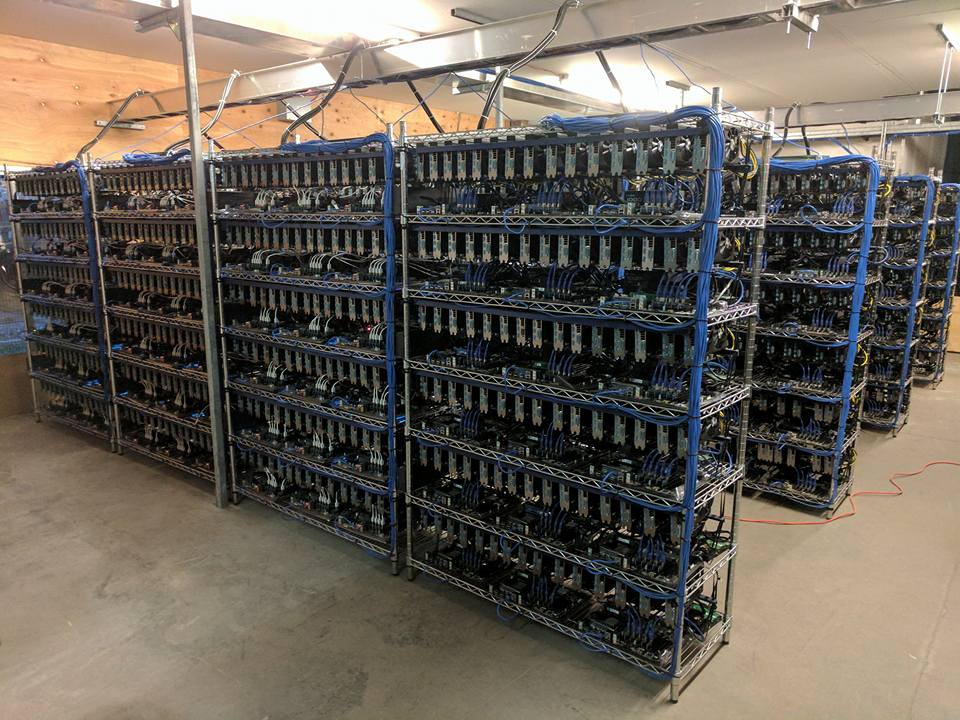
\includegraphics [width = 10cm] {ethfarm.jpeg}
\centering
\caption {Una \textit{farm} di Ethereum con 1440 schede grafiche}
\end{figure}
\vspace {0.2cm}
\noindent
%
Si verificò una vera e propria crisi nel mercato delle schede grafiche: i negozi erano quasi sempre vuoti, e appena arrivava un nuovo carico di GPU queste venivano istantaneamente acquistate.
Ovviamente i mercanti videro questa come un'opportunità per aumentare i profitti sulla loro merce, e così aumentarono esponenzialmente i prezzi di tutti i modelli di schede grafiche.
Per esempio le AMD RX 580 8GB con MSRP\footnote{\textit{Manufacturer's Suggested Retail Price}, il prezzo di un oggetto consigliato dal manufattore} pari a \euro{159} raggiunsero prezzi ben oltre \euro{300} \cite{ethboom}.
Questa inflazione è in corso tutt'oggi.


\subsection {Litecoin}


Litecoin (LTC) è una criptovaluta creata nell'ottobre del 2011 dallo sviluppatore Charles Lee, comunemente chiamato Charlie Lee. L'obiettivo di questa valuta è quello di relazionarsi al Bitcoin come l'argento fa con l'oro.
Come per questi metalli, infatti, l'oro è usato come uno \textit{store of value}\footnote{Riserva di valore}, essendo un metallo prezioso con elevato valore (oggi circa \euro{42} per grammo). L'argento è un metallo più comune con valore ben inferiore all'oro (oggi circa \euro{16} per grammo), usato anche dalle industrie.
Lo stesso vale per Bitcoin e Litecoin. Come abbiamo visto in precedenza la quantità totale di bitcoin è limitata a 21.000.000 BTC, e il valore attuale per bitcoin è di circa \euro{7000}.
Di litecoin invece ne possono esistere ben 84.000.000, e il prezzo per LTC è di \euro{100}.
Il tempo stabilito per trovare un nuovo blocco è di 2.5 minuti anziché 10, rendendo le transazioni notevolmente più veloci.
Per bilanciare la maggior quantità di litecoin che possono esistere, l'\textit{halving} avviene ogni 840.000 blocchi anziché ogni 210.000 \cite{ltcvsbtc}.


\subsection {Monero}


Monero (XMR) è un altcoin creato in aprile 2014 che ha come prima preoccupazione quella della privacy.
Monero è l'unica criptovaluta che è completamente intracciabile. Come abbiamo visto con il Bitcoin, nella blockchain possiamo trovare informazioni su tutto quello che avviene: il bilancio di qualunque indirizzo, chi manda quanto a chi.
Con Monero tutto questo non è possibile. Mentre ha una blockchain come tutti gli altri coin, non è possibile vedere le transazioni che avvengono dall'uno all'altro indirizzo, e non è nemmeno possibile visualizzare il saldo.

\vspace {0.5cm}
\begin{figure}[htb!]
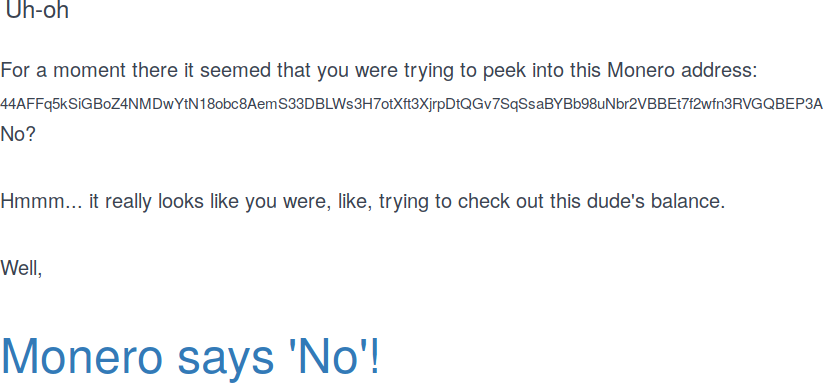
\includegraphics [width = 10cm] {monero.png}
\centering
\caption {Sul sito moneroblocks.info viene mostrato il seguente messaggio se si cercano informazioni legate a un indirizzo}
\end{figure}
\vspace {0.2cm}
\noindent
%
Questo rende Monero una valuta estremamente utile a chiunque voglia nascondere i propri fondi.
Purtroppo, come tutte le tecnologie a favore della privacy, Monero viene utilizzato anche da evasori delle tasse, truffatori e da venditori di merce illegale.
Monero ha un tempo stabilito di scoperta blocchi di 2 minuti, rendendo le transazioni relativamente veloci.
Inizialmente il tempo per trovare il blocco successivo era di 1 minuto, ma poi è stato aumentato a 2 minuti per ridurre la quantità di blocchi orfani e perché i blocchi non venivano sufficientemente "riempiti" di transazioni.
Le transazioni di Monero, per essere anonime, hanno un peso in kb notevole, per questo le tasse di transazione sono più elevate di quelle della maggior parte delle altre criptovalute. %quindi... quanto? quanto pesano?

\subsection {Nano}


Inizialmente chiamata RaiBlocks\footnote{il passaggio da RaiBlocks a Nano è avvenuto il 31 Gennaio 2018}, Nano è una criptovaluta creata nel MESE 2015 dallo sviluppatore Colin LeMahieu.
A differenza delle valute che dipendono da \textit{proof of work}, Nano non prevede l'impiego di miners per validare le proprie transazioni https://nano.org/en/faq.
sistma di representers... ecc. dovrei metterlo dopo?
Esistono in totale 133.248.290 NANO, distribuiti gratuitamente fino all'ottobre 2017 tramite un sito che inviava una piccola quantità di Nano a chiunque completasse un \textit{captcha}, una parola da trascrivere in una casella di testo per confermare di non essere un robot programmato per abusare del sistema di distribuzione gratuita.
È veramente interessante sotto il punto di vista tecnico perché è la prima che usa la tecnologia \textit{Block Lattice}\footnote{Da non confondere con la parola italiana, \textit{lattice [/'let.is/]} significa reticolo, intreccio} in sostanza, anziché dipendere da una singola blockchain come fanno tutte le altre valute, ogni singolo indirizzo \emph{è} una blockchain a sé stante.
Questa tecnologia permette di effettuare transazioni estremamente veloci rispetto a quelle del Bitcoin (che impiegano un'ora per essere ritenute pienamente concluse), con una durata inferiore ai 2 secondi, talvolta letteralmente istantanee.
Non è l'unico vantaggio. A differenzaaa
La \textit{Block Lattice} , poichè...SPIEGARE, rende tutte le transazioni di Nano completamente gratuite.


\subsection {Ripple}


Ripple (XRP) è un altcoin creato nel dalla Ripple Foundation.%(each transaction destroys a small amount XRP, is the supply of coins getting smaller?)
La sua particolarità sta nel fatto che Ripple mira ad essere una valuta fortemente legata all'ambito bancario, utilizzata come un bene digitale per compiere scambi di valore tra banche.
La principale critica a Ripple è quella di non essere decentralizzato come la stragrande maggioranza delle criptovalute, bensì la Ripple Foundation ha una forte influenza sull'andamento della valuta.
Ripple è un coin \textit{premined}, che non è generato tramite mining, infatti per entrarne in possesso è solamente possibile acquistarne direttamente dalla Foundation.
Per questo, la Ripple Foundation possiede oltre il 50\% di tutti i ripple, circa 50.000.000.000 XRP \cite{ripple}. Questo le permette di modificare artificialmente il prezzo.


\subsection {Bitcoin "hard forks"}


La blockchain del Bitcoin "originale" può essere clonata indefinitamente. Chiunque può prendere il codice sorgente del Bitcoin, applicarci qualche modifica e mandarlo "live", rendendo disponibili dei wallet al download e impiegando qualche miner per processare le transazioni del "nuovo" bitcoin.

\vspace {0.5cm}
\begin{figure}[htb!]
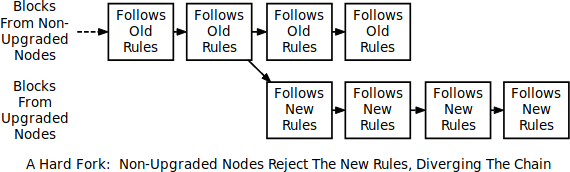
\includegraphics [width = 10cm] {hard_fork.png}
\centering
\caption {Schema di un'\textit{hard fork}: I \textit{full nodes} non aggiornati ignorano le nuove regole, dividendo in due la blockchain\\\textit{fonte: investopedia.com}}
\end{figure}
\vspace {0.2cm}
\noindent
%
Tecnicamente Litecoin è una \textit{hard fork} del Bitcoin, ma ho deciso di dedicarle un paragrafo a sé stante perché, a differenza delle altre di cui parlerò in seguito, Litecoin introduce numerose differenze e il nome non include la parola "Bitcoin".
Oggi esistono più di 30 \textit{fork} del Bitcoin: Bitcoin Gold, Bitcoin Candy, Bitcoin Private, Bitcoin Unlimited, Bitcoin Super... Persino Bitcoin Pizza e Bitcoin God.
Quasi tutti i fork vengono visti come delle truffe, come valute che non possiedono nulla di nuovo rispetto all'originale Bitcoin, ma viene sempre data attenzione perché chiunque possiede Bitcoin il momento in cui la blockchain è stata clonata, entra automaticamente in possesso del coin della fork.
Se un indirizzo ha il bilancio di X BTC \emph{prima} che venga lanciata la \textit{hard fork}, per esempio Bitcoin Top (BTT) a quell'indirizzo sarà anche associato X BTT.
Per poter ottenere effettivamente tutti i coin che l'indirizzo "possiede", è necessario scaricare il software di wallet del coin di fork e inserire la private key dell'indirizzo con su il coin di fork.
Verrà generato un nuovo indirizzo completamente diverso, però con il bilancio di X BTT.
Abbiamo visto prima che la private key dà accesso a tutti i fondi presenti sull'indirizzo a chiunque ne entri in possesso, eppure per ottenere i Fork siamo costretti ad inserirla in un software sconosciuto (perchè quasi tutti i fork non hanno alcuna reputazione: saltano fuori con siti web senza preavviso).
Per evitare che un qualche malintenzionato sfrutti la sbadataggine dell'utente e rubi tutti i suoi bitcoin, è bene che I fondi vengano mossi a un altro indirizzo.
Infatti, sarà comunque possibile prelevare i BTT dal vecchio indirizzo BTC ora svuotato, e non si ha nulla da perdere nel caso qualcuno riuscisse a rubare la private key: all'indirizzo sono associati 0 BTC.


\newpage


\section {Crypto oggi}


In questa sezione andrò a parlare dell'impatto del Bitcoin nella società di oggi.


\subsection {Adozione}


Il Bitcoin è una valuta relativamente nuova nata neanche 10 anni fa, e il fatto che utilizza una tecnologia sconosiuta prima d'ora, limita l'adozione da parte di mercanti e imprese.
Nonostante ciò, sempre più servizi stanno cominciando ad accettare criptovalute come forma di pagamento, tra cui:

\begin{itemize}
\item Immobiliare: in varie parti del mondo si stanno vendendo ville e appartamenti. A Dubai, per esempio, sono stati venduti 50 appartamenti di lusso per Bitcoin\cite{dubai}.
\item Microsoft: è possibile acquistare software e giochi sul Microsoft Store con Bitcoin \cite{accepting}.
\item Gyft e eGifter: è possibile comprare codici regalo per una moltitudine di siti che non accettano Bitcoin tra cui Amazon, iTunes, Nike, eBay e Starbucks \cite{accepting}. 
\item KFC Canada e Subway: due catene fast-food famose in tutto il mondo stanno incominciando ad accettare Bitcoin \cite{accepting}. 
\end{itemize}

Un fattore concreto che indica l'adozione del Bitcoin è il numero di transazioni giornaliere:

\vspace {0.5cm}
\begin{figure}[htb!]
\makebox [\textwidth] [c] {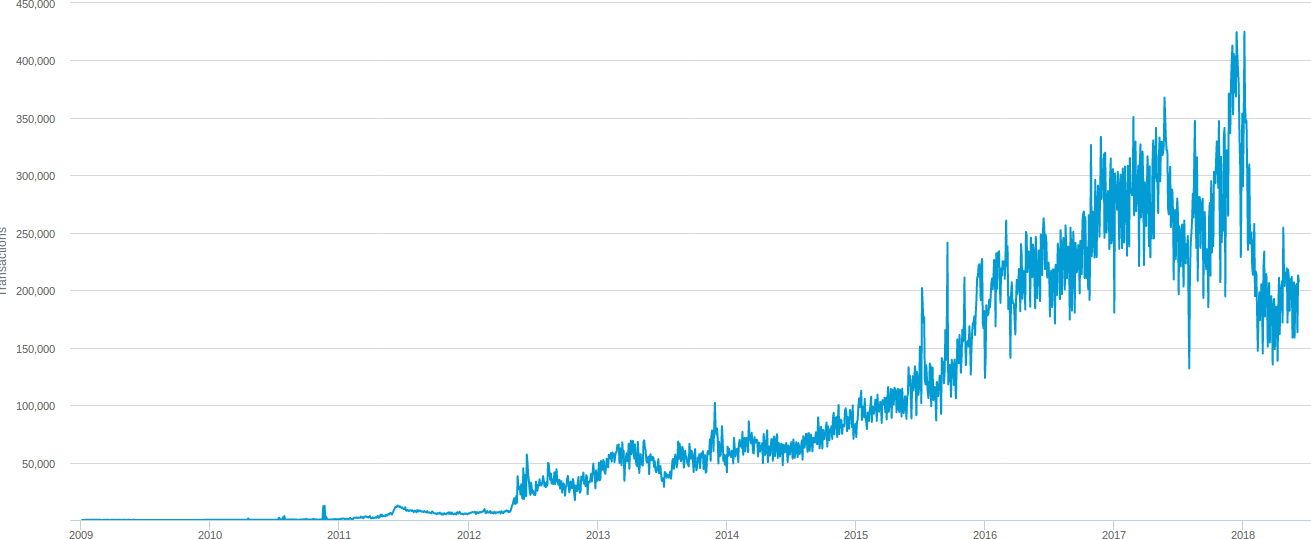
\includegraphics [width=15cm] {transactions.png}}
\caption {Transazioni giornaliere a partire dal 2009\\\textit{fonte: blockchain.info}}
\end{figure}
\vspace {0.2cm}
\noindent
%

\paragraph {Rovereto: quasi tutti accettano Bitcoin}

Rovereto è una cittadina nelle Dolomiti di 40.000 abitanti in cui l'uso del Bitcoin come forma di pagamento è estremamente diffusa.
Tutto ebbe inizio  quando ... ...
\cite{rovereto}


\paragraph {Elizavetovka: il villaggio in Ucraina in cui tutti utilizzano criptovalute}


è bellus \cite{elizavetovka}


\subsection {La bolla del 2017: cause e conseguenze}


A partire dal settembre 2017 il prezzo del Bitcoin ha subito un'esponenziale crescita, passando dai \euro{3000} del 16 settembre fino a raggiungere un picco di \euro{17.230} il 12 dicembre.
Le cose(?) che hanno causato questo boom non sono certe, ma
Il prezzo del Bitcoin, ma anche della stragrande maggioranza delle altre criptovalute è precipitato nel dicembre del 2017, andando dall'ATH (\textit{all time high}) del 12 dicembre di \euro{17.230} ai \euro{6000} del 5 Febbraio 2018. Un calo di più del 65\%!
futures?


\subsubsection {L'analogia con la crisi del '29}


Il 24 ottobre del 1929 è il giorno che marcò il crollo della Borsa di Wall Street, che ebbe come conseguenza il fallimento di molte imprese, una riduzione della domanda da parte di altri stati, e una forte crescita della disoccupazione, raggiungendo i 13 milioni di disoccupati nel 1932.
Tra le principali cause di questa crisi ci sono la sovrapproduzione di merce. detto così sembra fatto da un bambino delle elementari
Gli Stati Uniti erano grandi fornitori di merce e dané all'Europa, e il progressivo aumento della domanda ha portato gli USA ad incrementare la produzione industriale, grazie anche alla diffusione del Taylorismo e della generale innovazione tecnologica().
A partire dal 1926, però, l'Europa e poi il Giappone ridussero notevolmente la domanda agli Stati Uniti perché anche questi beneficiarono del progresso tecnologico che ha avuto inizio in America.
Questo portò a un'eccessiva produzione di merce che non venne mai venduta all'Europa perché non richiesta.
Un'altra enorme causa di questa crisi fu l'andamento dell'economia mondiale: era puramente un'economia di carta, basata su opinioni e speculazioni.
Gli scambi di azioni e gli investimenti di imprenditori verso le diverse aziende era una scommessa su quale attività avrebbe fatto successo, facendo ricavare profitti a chi avesse investito. \cite{crisi29}
Questo è estremamente simile a quello che è successo al Bitcoin perché sì.

\paragraph {La ricorrenza dei "crash" dei mercati}

\vspace {0.5cm}
\begin{figure}[htb!]
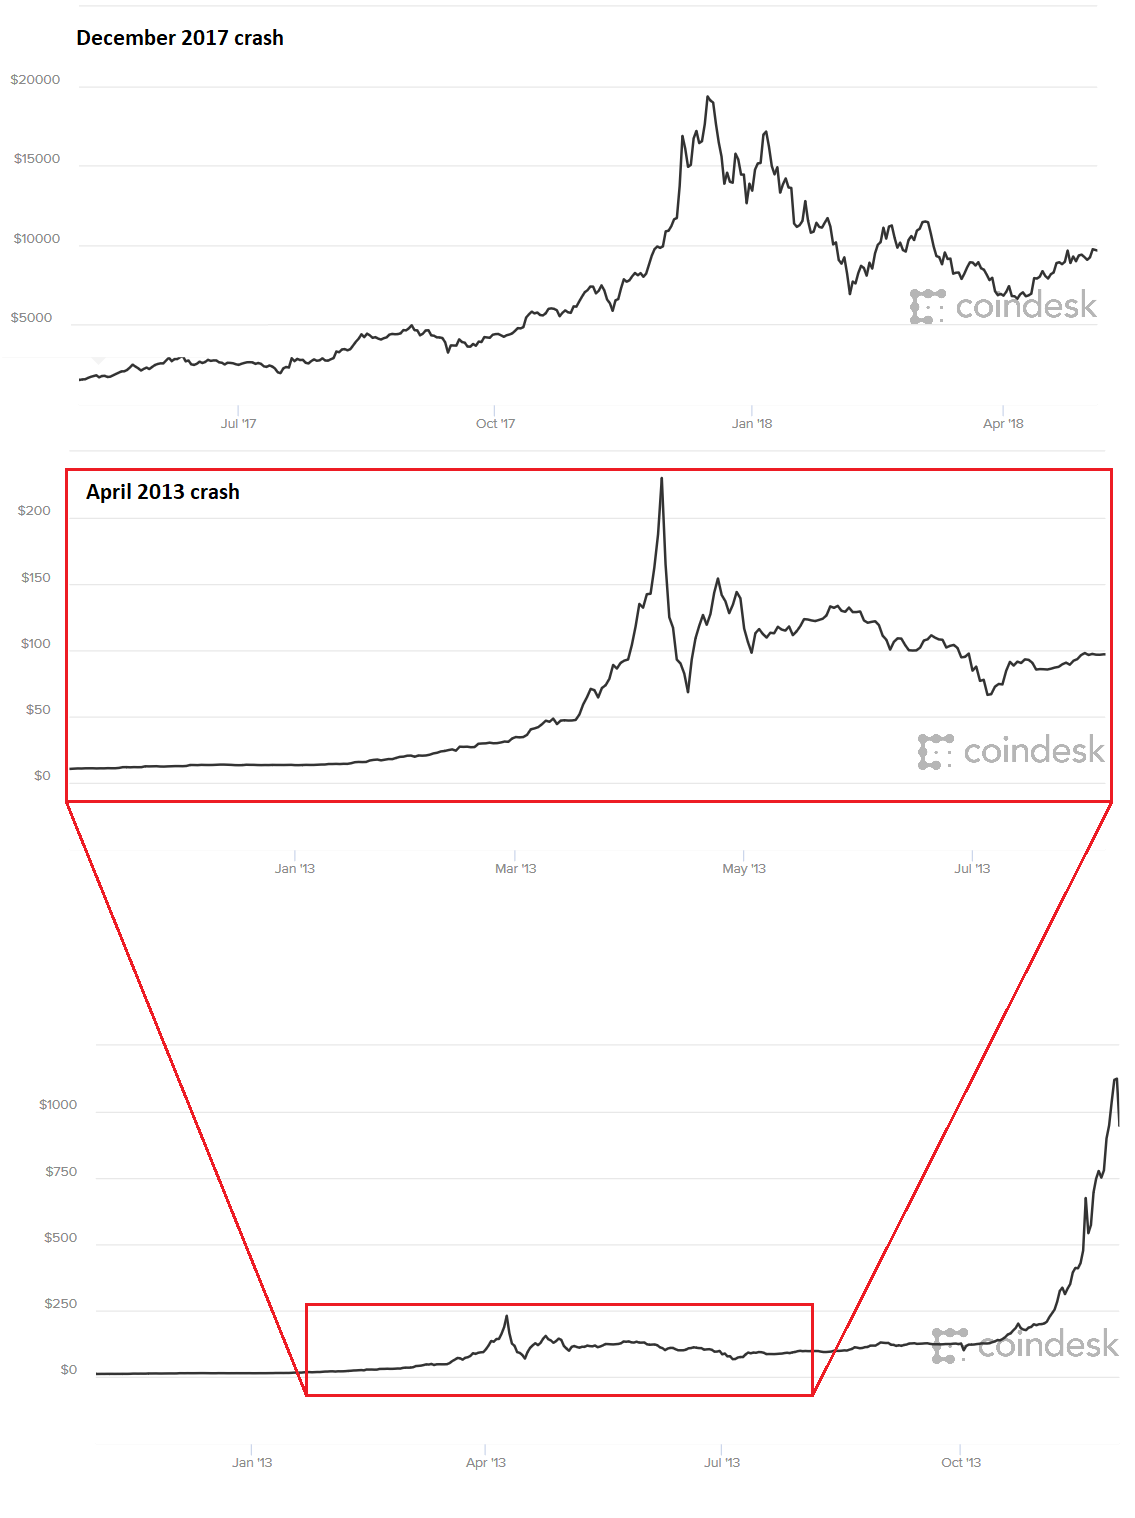
\includegraphics [width = 10cm] {crash2.png}
\centering
\caption {Confronto tra il crollo del prezzo del Bitcoin nel 2013 e nel 2017}
\end{figure}
\vspace {0.2cm}
\noindent
%

\subsection {Controversie}


Il Bitcoin e le criptovalute in generale sono frequentemente soggetto di controversie. La nuova tecnologia della blockchain è criticata da molti imprenditori, e numerosissime truffe girano intorno alla parziale anonimità della valuta \cite{controversy}.


\subsubsection {Moneta per scambi illegali}


Inizialmente il Bitcoin, ma oggi anche altre criptovalute (speciamente quelle centrate sulla privacy), sono usate per compiere scambi di merce proibita, principalmente droga e armi.
Nel deep/dark web, infatti, esistono numerosi siti dove è possibile acquistare merce illegale tramite criptovalute.
Fino al 2013, nei primi anni del Bitcoin, infatti, la valuta era quasi esclusivamente utilizzata per fare acquisti sul \textit{marketplace} chiamato Silk Road\footnote{Strada di seta}, chiuso dall'F.B.I. nel 20XX.
L'accusa alle criptovalute di essere monete "da mercato nero" è secondo molti una forma di FUD, \textit{fear, uncertainty, doubt}\footnote{Paura, incertezza, dubbio: tecnica per incutere timore nella gente inesperta riguardo a qualcosa}, per il semplice fatto che la moneta cartacea, il \textit{cash} è anch'essa una forma di denaro da sempre usata per atti/motivi illeciti, anch'essa anonima, più del Bitcoin! 


\subsubsection {Il ban del Bitcoin in certi stati}


boh, faccio dopo.


\subsubsection {Mt. Gox}


Mt. Gox è il primo grande sito di exchange di Bitcoin, creato a Tokyo nel 2013.
Ai tempi il Bitcoin aveva un valore ben più basso del \textasciitilde 9000 di oggi: il giorno in cui l'hack è avvenuto un bitcoin valeva solo \euro{500}. FINIRE


\subsubsection {Bitconnect}


Bitconnect è un altcoin con un tasso di interesse variabile (dal 0.1\% all'1\%) che aumentava quotidianamente i profitti di chiunque ne possedesse.
Non era ben chiaro chi fosse il creatore, e molti erano già dubiosi del claim di arricchire magicamente chiunque ne comprasse.
Tra il 14 e il 17 Gennaio 2018 il prezzo di Bitconnect è crollato da \euro{273} a \euro{30}, arrivando agli \euro{0.55} di oggi.
Si è scoperto che l'intero progetto Bitconnect non era altro che un' "exit scam", una truffa in cui i truffatori spariscono improvvisamente, lasciando gli investitori a mani vuote.
In particolare Bitconenct è stato uno schema Ponzi, un tipo di truffa in cui il truffatore promette guadagni a chiunque si indebitasse con lui, per poi sparire.
Il nome Ponzi deriva da Charles Ponzi, un italo-americano che si arricchì notevolmente tra il 1918 e il 1920 compiendo ripetutamente questo tipo di truffa.
Oggi tutti coloro coinvolti nel pubblicizzare Bitconnect, soprattutto chi pubblicava video su YouTube che incitavano all'acquisto della valuta, sono sotto investigazione.


\subsubsection {Roger Ver e la truffa di "Bitcoin Cash"}


Bitcoin Cash è di gran lunga l'hard fork più popolare di tutte, al quarto posto (!) in capitalizzazione di mercato. Come mai è l'unica che ha raggiunto un prezzo così elevato?
Roger K. Ver è un imprenditore americano che fin dai primi anni della nascita del Bitcoin è stato coinvolto nella scena delle criptovalute.
Dall'agosto del 2017, però, quando è stato lanciato Bitcoin Cash, Roger è stato l'esponente principale per il marketing di questa valuta. BCH è nato in Cina, infatti i suoi "CEO" sono cinesi, e Roger dev'essere stato impiegato per fare propaganda a BCH.
Tutto ciò non sembra alcunché di preoccupante: è normale se un imprenditore pubblicizza i propri investimenti sperando di ricavare più guadagni, (nel caso che...) ed è normale che sviluppatori paghnio uno abile a parlare e a pubblcizzare un prodotto.
è così che funziona il marketing.
Quella di Roger, però, è una spietata propaganda anti-Bitcoin (BTC) e pro-BCH (Bitcoin Cash), che spesso e volentieri arriva alla censura, alle bugie più false e alla corruzione di persone.
La tesi base che accomuna Roger e tutti i fan di BCH (pagati o no non si sa), è quella che BCH introduce delle modifiche al codice di Bitcoin che rendono le transizioni notevolmente più veloci, sicure e con una tassa di transazione inferiore. Bitcoin Cash infatti ha come principale differenza un'incrementata dimensione del blocco\footnote{Vedi punto X.X}, che anzichè limitarsi a 1MB arriva fino a 12MB% (come abbiamo visto, ogni transazione pesa tot kb. essendo il blocco più grande può farci stare più transazioni, senza "intasarsi").
Il team di sviluppatori di Bitcoin si ostina a mantenere la dimensione del blocco a 1MB, perchè i blocchi di maggiore dimensioni sono \emph{ancora} più difficili da minare.
Una difficoltà così elevata di mining porta necessariamente a una centralizzazione dell'hashing power, che va contro il concetto di Bitcoin e di criptovalute in generale. inoltre, .... \cite{bigblocks}
Roger è entrato in possesso del sito bitcoin.com, che su numerose pagine (tra cui quella in fig. 5) ripete come BCH è una versione aggiornata di BTC. Una cosa che irrita la stragrande maggioranza delle persone è il fatto che su bitcoin.com il Bitcoin originale, BTC, è chiamato Bitcoin Core.
Il nome Bitcoin Core, paragonato a Bitcoin Cash, fa sembrare le due valute due alternative sullo stesso livello, invece uno (BCH) è un clone dell'originale (BTC).
In Aprile del 2018 bitcoin.com penalizzò ulteriormente la situazione del "vero" Bitcoin definendo "BTC" "Bitcoin Core" e "BCH" (che sarebbe Bitcoin Cash) "Bitcoin".
Questa mossa fu la goccia che fece traboccare il vaso, perché mentre il fatto di chiamare BTC Bitcoin Core era già una bugia di per sé, sostituire "Bitcoin Cash" con "Bitcoin" era semplicemente inaccettabile.
A seguito di questa modifica dei termini, bitcoin.com venne denunciato da oltre 1000 persone e fu eventualmente costretto a tornare alle vecchie denominazioni delle valute che, purché volontariamente misleading, non facevano apparire BCH come il "vero" Bitcoin \cite{verlawsuit}.
bitcoin.com, essendo il secondo risultato su Google per la ricerca "bitcoin", ha portato molte persone nuove nel mondo delle criptovalute che cercavano di acquistare dei Bitcoin ad acquistare BCH anziché BTC.
Ver possiede anche l'account Twitter @bitcoin, che svolge le stesse opere di propaganda di bitcoin.com


\subsection {Il futuro delle criptovalute}


Molti ritengono che quella del Bitcoin sia solo una moda passeggera, simile a quella dei film in 3D e Google Glass, che ha avuto il suo picco nell'inverno del 2017 e che è destinato a sparire.
Personalmente sono ottimista nello sviluppo delle criptovalute.
Osservando l'andamento dei grafici, pur avendo subito gravi crolli in brevi intervalli di tempo, il prezzo delle valute è in una regolare crescita.
Il fatto che se ne parli sempre più nei media (i media parlino piu), sebbene spesso in negativo, rende la gente comune consapevole dell'esistenza di questa tecnologia, e fra tanti che la ignorano sono sicuro che qualcuno come me si interessi.
La natura deflazionaria della valuta aiuta sicuramente il prezzo: abbiamo visto che non possono esistere più di 21 milioni di bitcoin, e ciò rende un'inflazione del prezzo tecnicamente impossibile. paragone all'inizio btcoro?
Tutte le inflazioni sono dovute a un'eccessiva stampa di soldi cartacei, cosa che è impossibile nell'ambito delle criptovalute.

\newpage

\printbibliography[title = {Bibliografia}]
 

\end{document}
